 
\documentclass{article}
\usepackage[a4paper,]{geometry}
%\usepackage[export]{adjustbox}
\usepackage[utf8]{inputenc}
\usepackage[T1]{fontenc}
\usepackage{graphicx}
%\usepackage{titlepic}
\usepackage{mathtools}
\usepackage{amsmath}
\usepackage{amssymb}
\usepackage{amsfonts}
%\usepackage{accents}
%\usepackage{esvect}
\usepackage{subcaption}
\usepackage{multicol}
\usepackage{hyperref}
%\usepackage{enumitem}
\usepackage[makeroom]{cancel}
\linespread{1.3}
\usepackage{siunitx}
\sisetup{separate-uncertainty=true}

\newcommand{\E}[1]{\, \mathrm{e}{#1} \, }

\title{Misure Resistenza}
\author{Filippo Dal Farra \and Matteo Zandegiacomo Orsolina}
\date{25 Ottobre 2018}

\begin{document}

\maketitle

\newpage

\section{Introduzione}
L'obiettivo dell'esperienza di laboratorio \'e di ottenere una verifica sperimentale della legge di Ohm tramite la misura di una resistenza $R_x$ con metodi differenti.\\
La legge di Ohm afferma che: 
\begin{equation}
    V = R i
    \label{eq:Ohm}
\end{equation}
Conoscendo i valori di \textit{V} e di \textit{i} ed utilizzando la legge si calcola il corrispondente valore di \textit{R}. In particolare le misure sono state effettuate sfruttando due tester ICE come amperometro e voltmetro, prima in configurazione amperometro a monte e poi in configurazione amperometro a valle, di modo da poter poter confrontare e commentare i risultati ottenuti nelle due situazioni. In particolare non trattandosi di strumenti ideali, l'amperometro presentava una certa resistenza in serie che causava una differenza di potenziale ai capi dello strumento, mentre il voltmetro reale possiede una resistenza in parallelo che causa il passaggio di parte della corrente che dovrebbe andare alla resistenza da misurare. Si pu\'o quindi dire che il loro utilizzo alterava parzialmente il valore di resistenza $R_m$ misurato rispetto a quello corretto.\\
Inoltre \'e interessante riscontrare se la resistenza in esame fosse di un materiale ohmico o meno, osservando se la legge di Ohm fosse compatibile con i dati ottenuti.\\

\newpage

\section{Materiali e strumenti}

\begin{itemize}
  \item Due tester ICE
  \item Una resistenza di valore nominale $R_{n}= \SI{4700}{\ohm \pm 5\percent}$
  \item Fili di materiale conduttore
  \item Cavi "banana-banana"
  \item Breadboard
  \item Bobina precedentemente realizzata
  \item Multimetro digitale (DMM)
  \item Generatore di tensione variabile
\end{itemize}

\newpage

\section{Procedure di misura}
Primo passo di questa esperienza è stato quello di determinare il valore nominale della resistenza fornita tramite il codice colori stampato su di essa. Questo è il punto di partenza, dal quale poi con le misure eseguite in seguito dobbiamo essere in grado di dire se questa quantità è corretta oppure no. Una prima verifica di ciò è stato il calcolo della resistenza con l'uso del multimetro digitale in configurazione a quattro terminali. \\
Abbiamo quindi realizzato un circuito su breadboard sul quale poter effettuare ulteriori misure di resistenza seguendo lo schema fornito sulla scheda di laboratorio (e riprodotto in Fig \ref{fig:amp-volt}). Sono stati sfruttati due diversi tester ICE uno come amperometro ed uno come voltmetro. Il primo circuito realizzato è stato quello in configurazione amperometro a monte, nel quale cioè la corrente passa attraverso il primo tester ICE, che funge da amperometro, per poi passare nella resistenza incognita e nel voltmetro in parallelo ad essa.\\
Per procedere con le misure si è reso necessario individuare dei valori di fondo scala sia per l'amperometro che per il voltmetro. Questo valore rappresenta la quantit\'a per la quale il tester analogico mostra la massima escursione della lancetta senza danneggiarsi. Come prima coppia di valori abbiamo scelto di usare come fondo scala del voltmetro un valore \textit{$ V_{FS} = 10V$} mentre per l'amperometro \textit{$i_{FS} = 5mA$}. Dopo aver realizzato dieci misure abbiamo cambiato i valori del fondo scala, scegliendo in questo caso per il voltmetro un \textit{$ V_{FS} = 2V$} mentre per l'amperometro un \textit{$i_{FS} = 0.5mA$}. Nel nostro caso utilizzare la seconda coppia di valori \'e stato pi\'u vantaggioso in quanto $2V/R_n \approx 0.4 \si{\milli\ampere}$ per cui abbiamo potuto sfruttare entrambi gli strumenti oltre alla met\'a del fondo scala, il che riduce l'incertezza relativa sulle misure, invece di fare un compromesso ed avere solo uno dei due oltre la met\'a. Infatti nel primo caso avevamo $10V/R_n \approx 2 \si{\milli\ampere}$ e cioò vuol dire che questo era il valore massimo che ci potevamo aspettare, di gran lunga inferiore al valore del fondo scala.\\
Siamo poi passati alla configurazione amperometro a valle, nella quale il voltmetro misura la tensione ai capi del \textit{parallelo} della resistenza $R_x$ e $R_A$. Anche in questo caso le misure sono state prese con le due coppie di valori di fondo scala precedentemente esposti.\\ \\
In seguito siamo passati alla misurazione della resistenza della bobina, la quale viene eseguita una sola volta con il circuito in configurazione amperometro a monte il quale in questo frangente \'e migliore di quello con amperometro a valle in quanto la $R_v$ interna del voltmetro \'e molto maggiore della $R_x$ della bobina ed essendo in parallelo la resistenza risultante \'e molto vicina al valore $R_x$.\\
Tale misura viene quindi confrontata con quella fornita dal DMM e dal calcolo teorico effettuato conoscendo resistivit\'a e geometria della bobina.

\newpage

%%%%%%%%%%%%% ANALisi %%%%%%%%%%%%%%%%%%%

\section{Analisi dei dati}

La resistenza fornita presenta un valore nominale pari a:
\begin{gather}
    R_n = \SI{4700(235)}{\ohm} \\
    \nonumber
    R_{n\ min} = \SI{4465}{\ohm} \quad
    R_{n\ max} = \SI{4935}{\ohm}
\end{gather}

Infatti sulla resistenza è segnalato il valore centrale con una tolleranza del $5\%$. Ciò vuol dire che il valore nominale $R_n$ può variare del $\pm 5\%$.

Viene quindi ora misurata con il multimetro digitale in configurazione a quattro terminali il quale ci fornisce il valore con un'incertezza la quale è stata determinata grazie al suo datasheet:
\begin{gather}
    R_{DMM} = \SI{4596.5}{\ohm \pm 100 ppm} \\
    \nonumber
    R_{DMM\ min} = \SI{4595.54}{\ohm} \quad
    R_{DMM\ max} = \SI{4596.46}{\ohm}
\end{gather}

Il valore ottenuto appartiene all'intervallo di accettazione entro $3 \sigma[R_n]$ dal valore nominale e la misura \'e pertanto compatibile con esso. \\
Prima di procedere a misurare la corrente attraverso i diversi circuiti abbiamo bisogno di capire qual è la differenza di potenziale massima che si pu\'o applicare alla resistenza sapendo il valore della potenza massima che \'e in grado di dissipare per effetto Joule senza che si danneggi, il quale ci è stato fornito.
\begin{equation}
    P_{max} = 0.5\ \si{\watt}
\end{equation}
\begin{equation}
    V_{max} = \sqrt{P_{max}R_{n}}\ \approx \SI{48}{\volt}
\end{equation}
Sappiamo quindi il valore oltre al quale non dobbiamo mai andare per evitare di alterare le proprietà della resistenza. Le misure tuttavia sono state effettuate con tensioni molto minori per limitazione del generatore fornito. \\
Sono stati quindi utilizzati i circuiti con i tester ICE per ottenere quattro serie di misure: due per circuito entrambe con due coppie di valori di fondo scala degli strumenti differenti. Si indicano con $V_i$ i valori ottenuti delle diverse differenze di potenziale e con $i_i$ i valori delle diverse correnti. Le grandezze che abbiamo misurato sono esposte nelle seguenti tabelle. Le incertezze relative ai diversi valori sono prese considerando solo gli errori di risoluzione. In particolare abbiamo ritenuto di essere in grado di distinguere solo la tacca intera sul lettore analogico di corrente e voltaggio. Per trovare l'intervallo di incertezza di ogni singola misura siamo partiti dall'assunzione che ogni valore può appartenere all'intervallo con la stessa probabilità per ogni punto. Perciò ciascun intervallo di risoluzione è stato diviso per $\sqrt{12}$, così da poter ottenere il corretto intervallo di incertezza $\sigma[V]$ e $\sigma[i]$.

\begin{figure}
\begin{center}
    \large{Amperometro a monte}
\end{center}
\begin{multicols}{2}
\begin{center}
\begin{tabular}{c|c} 
$V_{FS}=\SI{10}{\volt}$&$i_{FS}=\SI{5}{\milli\ampere}$\\
$V_i \pm \sigma [V]$ [\si{\volt}] & $i_i \pm \sigma [i]$ [\si{\milli\ampere}]\\
[0.5ex]
\hline
$9.6 \pm 0.06 $&$2.2 \pm 0.03$\\

$7.8 \pm 0.06 $&$1.7 \pm 0.03$\\

$8.6 \pm 0.06 $&$1.9 \pm 0.03$\\

$8.6 \pm 0.06 $&$1.8 \pm 0.03$\\

$7.2 \pm 0.06 $&$1.5 \pm 0.03$\\

$7.2 \pm 0.06 $&$1.6 \pm 0.03$\\

$5.6 \pm 0.06 $&$1.2 \pm 0.03$\\

$6.0 \pm 0.06 $&$1.3 \pm 0.03$\\

$8.0 \pm 0.06 $&$1.7 \pm 0.03$\\

$8.8 \pm 0.06 $&$1.9 \pm 0.03$\\

\end{tabular}
\end{center}

\begin{center}
\begin{tabular}{c|c} 
$V_{FS}=\SI{2}{\volt}$&$i_{FS}=\SI{500}{\micro\ampere}$\\
$V_i \pm \sigma [V]$        [\si{\volt}] & $i_i \pm \sigma [i]$         [\si{\milli\ampere}]\\
[0.5ex]
\hline
$1.80 \pm 0.01 $& $0.43 \pm 0.003$\\
$1.36 \pm 0.01 $&$0.33 \pm 0.003$\\

$1.40 \pm 0.01 $&$0.34 \pm 0.003$\\

$1.64 \pm 0.01 $&$0.39 \pm 0.003$\\

$1.52 \pm 0.01 $&$0.37 \pm 0.003$\\

$1.56 \pm 0.01 $&$0.38 \pm 0.003$\\

$1.20 \pm 0.01 $&$0.29 \pm 0.003$\\

$1.92 \pm 0.01 $&$0.46 \pm 0.003$\\

$1.76 \pm 0.01 $&$0.43 \pm 0.003$\\

$1.68 \pm 0.01 $&$0.40 \pm 0.003$\\

\end{tabular}
\end{center} 
\end{multicols}

\begin{center}
    \large{Amperometro a valle}
\end{center}
\begin{multicols}{2}
\begin{center}
\begin{tabular}{c|c} 
$V_{FS}=\SI{10}{\volt}$&$i_{FS}=\SI{5}{\milli\ampere}$\\
$V_i \pm \sigma [V]$ [\si{\volt}] & $i_i \pm \sigma [i]$ [\si{\milli\ampere}]\\
[0.5ex]
\hline
$9.8 \pm 0.06 $&$2.1 \pm 0.03$\\

$9.2 \pm 0.06 $&$2.0 \pm 0.03$\\

$8.6 \pm 0.06 $&$1.8 \pm 0.03$\\

$7.4 \pm 0.06 $&$1.6 \pm 0.03$\\

$6.4 \pm 0.06 $&$1.3 \pm 0.03$\\

$7.2 \pm 0.06 $&$1.6 \pm 0.03$\\

$7.8 \pm 0.06 $&$1.7 \pm 0.03$\\

$5.8 \pm 0.06 $&$1.2 \pm 0.03$\\

$6.4 \pm 0.06 $&$1.3 \pm 0.03$\\

$8.2 \pm 0.06 $&$1.7 \pm 0.03$\\

\end{tabular}
\end{center} 

\begin{center}
\begin{tabular}{c|c} 
$V_{FS}=\SI{10}{\volt}$&$i_{FS}=\SI{500}{\micro\ampere}$\\
$V_i \pm \sigma [V]$ [\si{\volt}] & $i_i \pm \sigma [i]$ [\si{\milli\ampere}]\\
[0.5ex]
\hline
$1.88 \pm 0.01 $&$0.36 \pm 0.003$\\

$1.72 \pm 0.01 $&$0.33 \pm 0.003$\\

$1.60 \pm 0.01 $&$0.31 \pm 0.003$\\

$1.36 \pm 0.01 $&$0.26 \pm 0.003$\\

$1.40 \pm 0.01 $&$0.27 \pm 0.003$\\

$1.96 \pm 0.01 $&$0.37 \pm 0.003$\\

$1.80 \pm 0.01 $&$0.35 \pm 0.003$\\

$1.52 \pm 0.01 $&$0.29 \pm 0.003$\\

$1.64 \pm 0.01 $&$0.31 \pm 0.003$\\

$1.48 \pm 0.01 $&$0.28 \pm 0.003$\\

\end{tabular}
\end{center}
\end{multicols}
\end{figure}

\newpage
I dati raccolti sono riassunti nei grafici in Fig. \ref{fig:quattro} i quali espongono \textit{visivamente} la relazione che ci aspettiamo, cio\'e proporzionalit\'a lineare tra la corrente $i$ e voltaggio $V$ nei singoli set di dati secondo la legge \ref{eq:Ohm}.\\

\begin{figure}[t]
    \centering
    \begin{minipage}{0.5\textwidth}
        \centering
        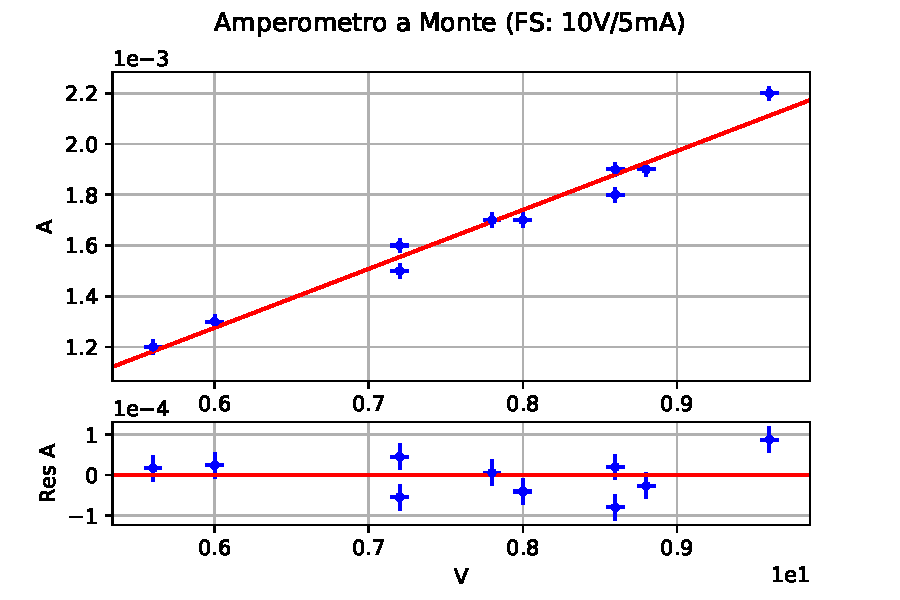
\includegraphics[width=\textwidth]{data/AmpMon10V5mA.pdf} 
        %\caption{first figure}
    \end{minipage}\hfill
    \begin{minipage}{0.5\textwidth}
        \centering
        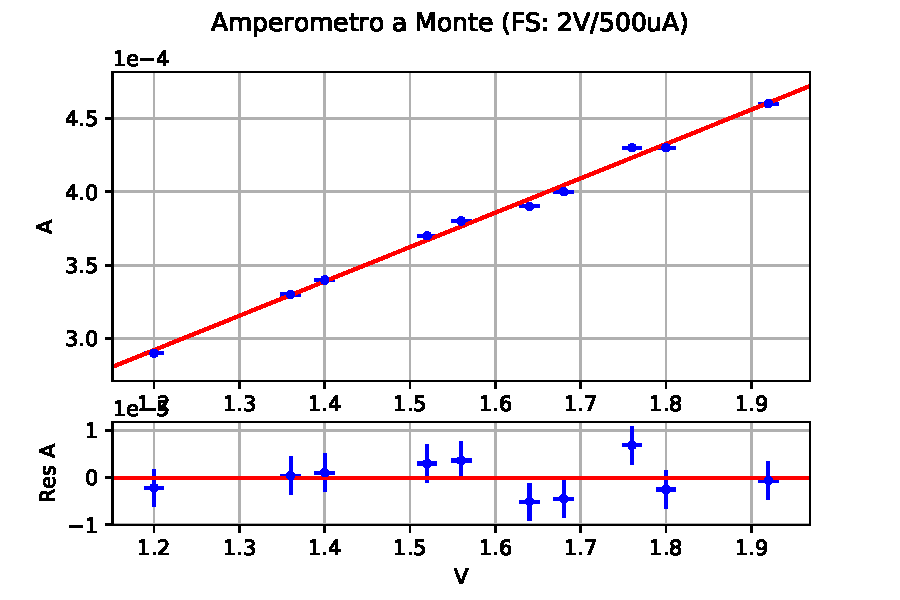
\includegraphics[width=\textwidth]{data/AmpMon2V500uA.pdf} 
        %\caption{second figure}
    \end{minipage}
    \\
    \centering
    \begin{minipage}{0.5\textwidth}
        \centering
        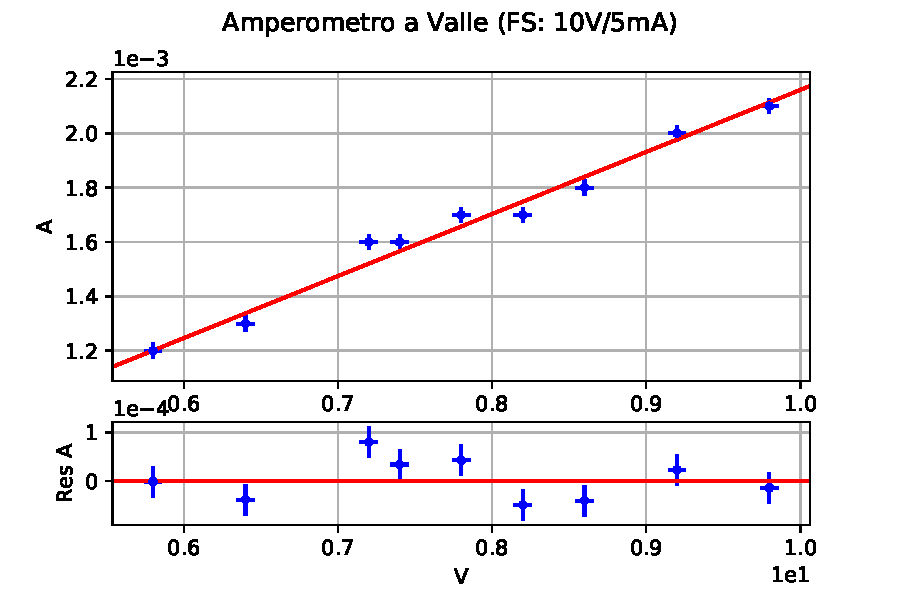
\includegraphics[width=\textwidth]{data/AmpVal10V5mA.pdf} 
        %\caption{first figure}
    \end{minipage}\hfill
    \begin{minipage}{0.5\textwidth}
        \centering
        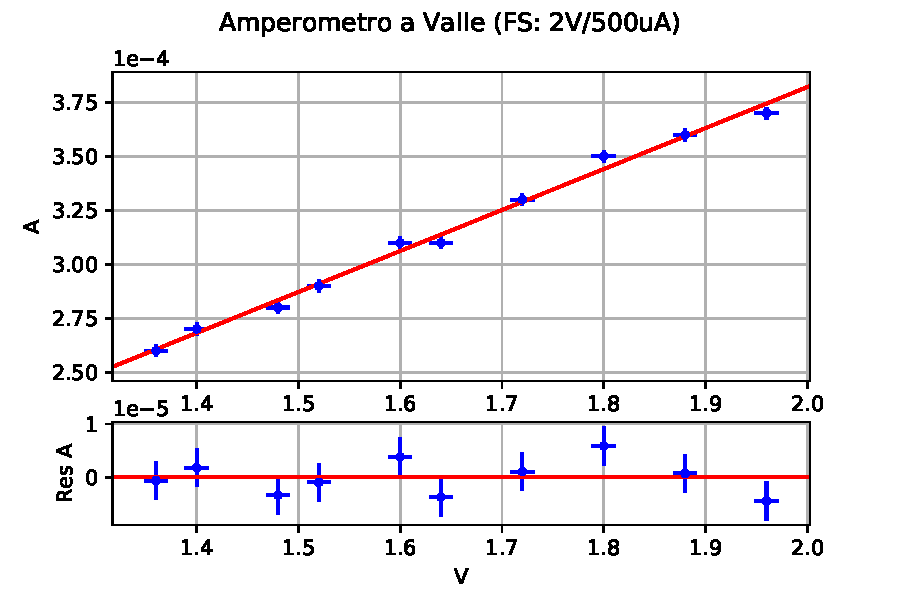
\includegraphics[width=\textwidth]{data/AmpVal2V500uA.pdf} 
        %\caption{second figure}
    \end{minipage}
    \caption{Grafici dei quattro set di dati accostati al modello calcolato su di essi}
    \label{fig:quattro}
\end{figure}

Ogni grafico rappresenta un set di dati in plot di tipo errorbar (in \textit{blu}) a confronto diretto con la regressione lineare (in \textit{rosso}) del tipo $y=A+Bx$. I grafici vanno considerati a coppie, uno relativo all'andamento che ci aspettiamo, accompagnato dal relativo grafico dei residui. Sul grafico superiore si ha sulle ascisse il voltaggio e sulle ordinate la corrente misurate dai tester ICE. Sul grafico sottostante sono invece mostrati gli scarti dal modello suddetto per meglio esprimere lo scostamento dai singoli sample.\\
Vengono quindi confrontati i quattro set nella Fig. \ref{fig:confr} dalla quale si nota una notevole differenza nelle intercette con l'asse y tra i set con i valori fondo scala minori e maggiori, mentre le misure prese con gli stessi valori di fondo scala presentano invece pendenze differenti.

\begin{figure}[ht]
	\centering
	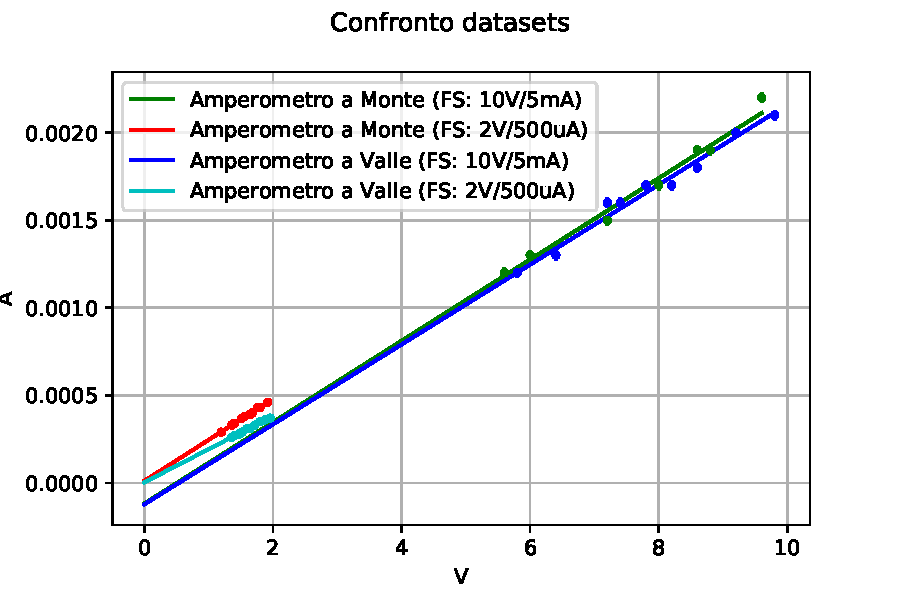
\includegraphics[width=0.8\textwidth]{data/FigAll.pdf}
	\caption{\label{fig:confr}}
\end{figure}
\newpage
La prima discrepanza pu\'o essere spiegata dal fatto che i valori misurati con fondo scala maggiore sono stati scelti volutamente mediamente pi\'u lontani dall'origine in modo da ridurre l'errore relativo sugli stessi.\\
Nel secondo caso invece la pendenza \'e differente in quanto \textit{in essa} \'e contenuta l'informazione sulla resistenza misurata, infatti:
\begin{equation}
	R_m=1/B
\end{equation}

Tuttavia, a seconda del circuito, la relazione tra $R_m$ e $R_x$ \'e differente per via della non idealit\'a dei tester ICE: il voltmetro non \'e un circuito aperto, come l'amperometro non \'e un corto circuito. Infatti entrambi sono schematizzabili come in Fig. \ref{fig:amp-volt} in cui il voltmetro ideale ha in parallelo una resistenza $R_V$ non infinita mentre l'amperometro ideale ha in serie una resistenza $R_A$ non nulla.

\begin{figure}[ht]
	\centering
	 \begin{minipage}{0.5\textwidth}
	     \centering
	     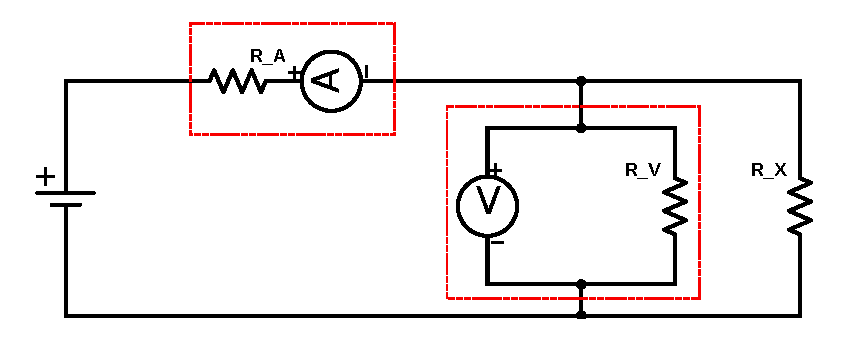
\includegraphics[width=\textwidth]{data/Amperometro_Monte.pdf} 
	     %\caption{first figure}
	 \end{minipage}\hfill
	 \begin{minipage}{0.5\textwidth}
	     \centering
	     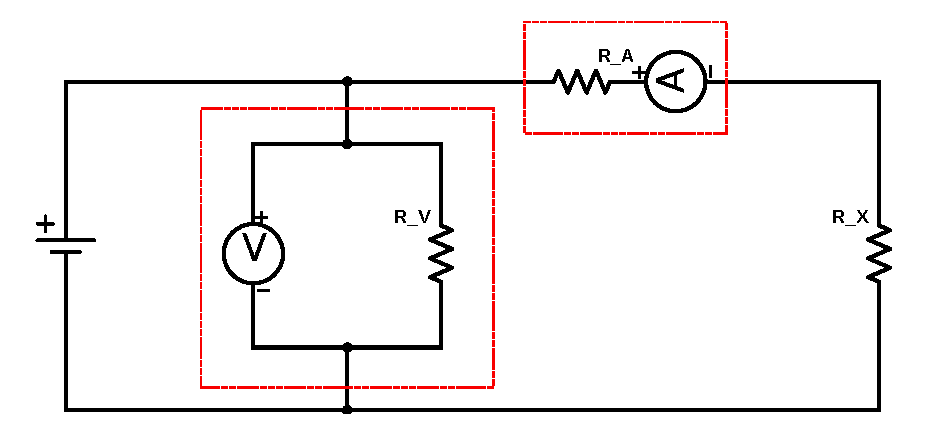
\includegraphics[width=\textwidth]{data/Amperometro_Valle.pdf} 
	     %\caption{second figure}
	 \end{minipage}
	 \caption{\label{fig:amp-volt}}
\end{figure}

\newpage

Risulta quindi che per avere i valori $R_x$ desiderati si ricorre all'applicazione delle formule per le resistenze in serie e in parallelo e si ottiene:
\begin{gather}
	\nonumber \mathrm{Amperometro\ a\ monte:} \\
	R_x=\frac{1}{B-\frac{1}{R_v}} \qquad \sigma[R_x]=\left|-\frac{1}{ \left(B-1/R_v\right) ^2 }\right| \sigma[B] \\
	\nonumber \mathrm{Amperometro\ a\ valle:} \\
	R_x=1/B - R_a \qquad \sigma[R_x] = \left|-\frac{1}{ B ^2 }\right| \sigma[B]
\end{gather}

Si procede quindi a calcolare un valore unico di resistenza $R_w$ come unione degli $R_x$ dei diversi set di dati tramite il calcolo della media pesata come segue:

\begin{gather}
	R_w = \frac{\sum{w_i R_{x\, i}}}{\sum{w_i}} \qquad w_i = \frac{1}{\sigma[R_{x\, i}]^2} \\
	\nonumber
	\sigma[R_w] = \sqrt{\frac{1}{\sum{w_i}}}
\end{gather}

I risultati di tutte le misurazioni sono posti a confronto nel grafico in Fig \ref{fig:comp}.

\begin{figure}[h]
	\centering
   	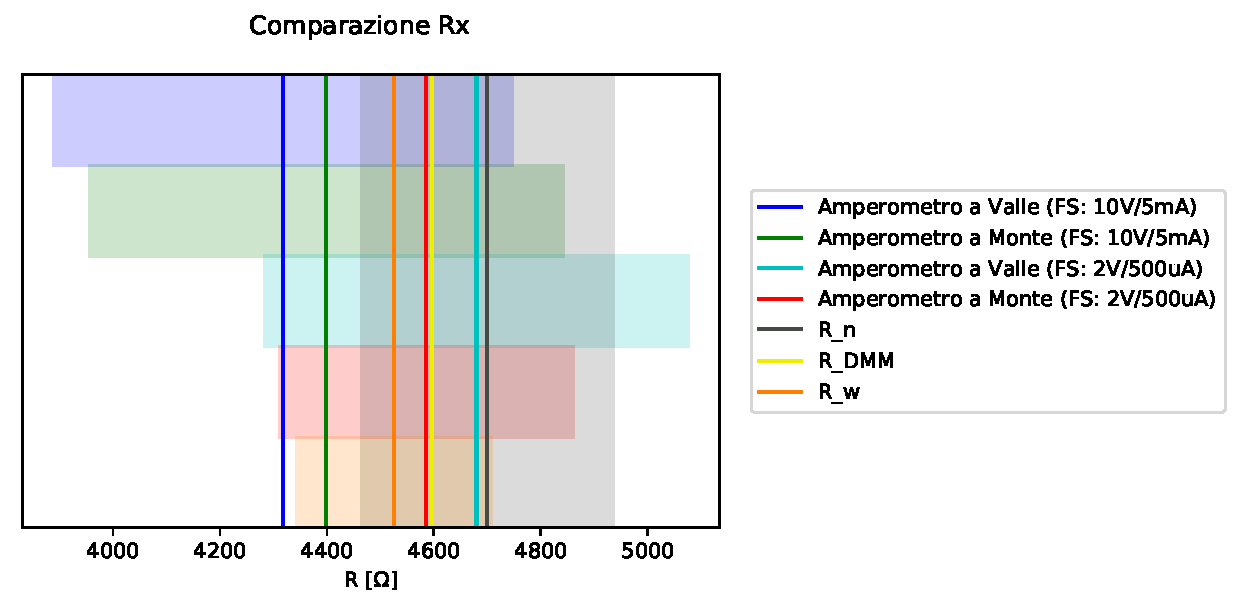
\includegraphics[width=\textwidth]{data/fig_comp.pdf} 
   	\caption{\label{fig:comp} In ascissa sono rappresentati i valori di resistenza. Gli span orizzontali rappresentano la distanza dal valore centrale di $3\, \sigma[R]$ e sono posti ad altezze differenti per evitare sovrapposizioni.}
\end{figure}

Come si pu\'o vedere i quattro set di misure sono tutti compatibili tra di loro entro $3\, \sigma$ il che giustifica l'aver utilizzato la media pesata per estrapolare un valore unico $R_w \pm \sigma[R_w]$.\\
Si osserva sia dalla Fig. \ref{fig:confr} che dalla Fig. \ref{fig:comp} che per le misure aventi fondo scala pi\`u alto deve esserci la presenza di un qualche errore sistematico. Infatti nel primo grafico si nota che le rette del modello in questa configurazione non passano per l`origine. Nel secondo grafico invece si vede che i loro intervalli sono maggiormente distaccati da $R_w$ rispetto a quelli provenienti dall'utilizzo del fondo scala minore. Ci\`o potrebbe essere spiegato con la presenza di un errore di taratura del tester ICE per quel particolare fondo scala.\\

\hspace{-2cm}
\vspace{12pt}
\begin{tabular}{c|c|c|c|c|c|c|c|c}
	& $V_{FS} [\si{\volt}]$ & $i_{FS} [\si{\milli\ampere}]$ & $R_A [\si{\ohm}]$ & $R_V [\si{\ohm}]$ & $A [\si{\milli\ampere}]$ & $B [\si{\per\ohm}]$ & $R_x [\si{\ohm}]$ & $\chi ^2_{r,\mathrm{dof}=8}$ \\
	\hline
	Monte 
	& 10 & 5 &  & $2 \E{5}$ & $0.12 \pm 0.06$ & $(2.32 \pm 0.08)\E{-4}$ & $(4.40 \pm 0.15)\E{3}$ & $2.8$ \\
	& 2 & 0.5 &  & $4 \E{4}$ & $(-3 \pm 7)\E{-3}$ & $(2.43 \pm 0.04)\E{-4}$ & $(4.59\pm0.09)\E{3}$ & $1.7$ \\
	Valle 
	& 10 & 5 & $63.5$ &  & $0.12 \pm 0.06$ & $(2.28 \pm 0.07)\E{-4}$ & $(4.32 \pm 0.14)\E{3}$ & $2.1$ \\
	& 2 & 0.5 & $588.8$ &  & $(2 \pm 8)\E{-3}$ & $(1.90 \pm 0.05)\E{-4}$ & $(4.68\pm0.13)\E{3}$ & $0.96$
\end{tabular}

Assumendo ora una probabilit\'a di falso allarme dell' $1 \%$ in un test del $\chi^2$ one-sided si ottiene che il primo set di dati non soddisfa la compatibilit\'a, tuttavia guardando il grafico in alto a sinistra in Fig. \ref{fig:quattro} si pu\'o notare come il valore avente ascissa ed ordinata maggiore sia il pi\'u distante dal modello. Dato che la legge che stiamo supponendo di tipo lineare non \'e incompatibile gli atri set di dati ed i residui sono distribuiti casualmente attorno al modello possiamo dire che potrebbe esserci stato un errore di lettura sulla scala del tester o di trascrizione. Si procede quindi all'eliminazione di questo dato ed al ricalcolo del fit e quindi del $\chi^2$ che ora presenta un valore $\chi^2_{r,\mathrm{dof}=7}=1.6$ il quale rientra nell'intervallo di accettazione data la probabilit\'a di falso allarme dell' $1\%$. Tuttavia dato che non c'è la certezza sia stato un errore triviale si mantengono i valori di $R_x$ precedentemente calcolati che comunque mantengono la compatibilit\'a con la misurazione effettuata con il DMM, di molto la pi\'u precisa a nostra disposizione.\\

Si riassumono quindi i risultati ottenuti con le varie tecniche nella seguente tabella e nel grafico \ref{fig:comp} gi\'a discusso.\\

\begin{center}
\begin{tabular}{c|c|c|c|c}
	& $V_{FS} [\si{\volt}]$ & $i_{FS} [\si{\milli\ampere}]$ & $R_x [\si{\ohm}]$ & $\chi ^2_{r,\mathrm{dof}=8}$ \\
	\hline
	Monte 
	& 10 & 5 & $(4.40 \pm 0.15)\E{3}$ & $2.8$ \\
	& 2 & 0.5 & $(4.59 \pm 0.09)\E{3}$ & $1.7$ \\
	Valle 
	& 10 & 5 & $(4.32 \pm 0.14)\E{3}$ & $2.1$ \\
	& 2 & 0.5 & $(4.68 \pm 0.13)\E{3}$ & $0.96$ \\
	$R_{DMM}$ &  &  & $4596 \pm 0.46$ &  \\
	$R_n$ &  &  & $(4.7 \pm 0.235) \E{3}$ & 
\end{tabular}
\end{center}

%\newpage

La bobina realizzata nella precedente esperienza \'e ora stata misurata con la configurazione Amperometro a Monte con i tester ICE e con la misurazione a quattro terminali del DMM ed i risultati che abbiamo ottenuto sono esposti nella seguente tabella assieme al calcolo teorico da noi precedentemente effettuato.

\begin{equation}
    R = \frac{\rho_{Cu} l}{S} = \frac{\rho_{Cu} (2 \pi r_{rocchetto} \ + \ 2 l_{filo extra})}{S_{filo}} = \frac{1.68\E{-8}\Ohm m \times (2 \pi \times 8.75\E{-3} \ + \ 2 \times 0.23)m}{7.79\E{-8}m^2}
\end{equation}

\begin{center}
\begin{figure}[h]
\centering
\begin{tabular}{c|c|c|c}
	& $V [\si{\volt}]$ & $i [\si{\milli\ampere}]$ & $R [\si{\ohm}]$\\
	\hline
	Tester ICE Amp. a Monte & 0.16 & 311 & $0.549$ \\
	DMM & 0.096 & 170 & $0.56 \pm 0.04$\\
	Calcolato & / & / & $0.49$
	
\end{tabular}
\caption{Risultati misurazioni della bobina}
\end{figure}
\end{center}
Osserviamo che il valore calcolato teoricamente si discosta parecchio dai valori calcolati, i quali fra loro risultano coincidenti. Ciò si può spiegare considerando che il valore teorico è stato calcolato considerando l'idealità del filo, il quale cioè non dovrebbe avere deformazioni o malfunzionamenti, oltre al fatto che è plausibile che le grandezze da noi misurate manualmente non siano state prese nel modo corretto. \\
Per effettuare queste misure abbiamo preso valori di voltaggio e corrente sufficientemente bassi da non danneggiare la bobina. Infatti dovevamo stare attenti che essa non si surriscaldasse troppo e che quindi non fossimo la causa di alcuni malfunzionamenti nel suo uso. Ci è stato dato come valore di densità di corrente massima $J_{max} = 4A/mm^2$ da cui si ottiene $I_{max}$
\begin{equation}
    I_{max} = j_{max} S_{filo} = \ 4A/mm^2 \times 0.158mm^2 \ = \ 0.311 A
\end{equation}
Infatti siamo stati ben attenti a non andare mai al di sopra di questo valore.

\newpage

\section{Conclusioni}
Siamo riusciti a trovare un valore della resistenza che ci era stata fornita compatibile e in particolare abbiamo osservato che inserita in un grafico essa rispetta un andamento lineare come predetto dalla legge di Ohm. Perciò possiamo affermare che la nostra resistenza fosse stata realizzata con un materiale ohmico. Tutte le misure inoltre risultano compatibili, perciò possiamo affermare che la legge di Ohm è un modello corretto per rappresentare il fenomeno.\\
Per quanto riguarda la bobina invece siamo stati in grado di trovare la sua resistenza attraverso diversi metodi, dimostrando che il valore teorico da noi predetto non era corretto a causa di probabili errori di misura da parte nostra, non quantificabili. Però la misura effettuata con due strumenti diversi si è rivelata compatibile fra loro, per cui abbiamo ottenuto un suo valore plausibile.
\end{document}
